\documentclass{article}
\usepackage[utf8]{inputenc}
\usepackage{graphicx}
\usepackage{listings}
\usepackage{color}
\usepackage{hyperref}
\hypersetup{colorlinks=true,
		urlcolor=blue}

\definecolor{mygreen}{rgb}{0,0.6,0}
\definecolor{mygray}{rgb}{0.5,0.5,0.5}
\definecolor{mymauve}{rgb}{0.58,0,0.82}

\lstset{
	basicstyle=\footnotesize,
	breaklines=true,
	captionpos=b,
	commentstyle=\color{mygreen},
	keywordstyle=\color{blue},
	stringstyle=\color{mymauve},
}

\begin{document}

    \title{Abstract Classes and Interfaces: Practical Examples}
    \author{Andrew Lalis | \emph{a.lalis@student.rug.nl} \\
            George Argyrousis | \emph{g.argyrousis@rug.nl} }
    \date{Last modified: \today}

    \maketitle

    \section{Abstract Classes}
        \subsection{Definition}
        	\href{https://docs.oracle.com/javase/tutorial/java/IandI/abstract.html}{Oracle Abstract Classes and Methods Tutorial}

            An abstract class, in the context of Java, is a superclass that cannot be instantiated and is used to state or define general characteristics. An object cannot be formed from a Java abstract class; trying to instantiate an abstract class only produces a compiler error. The abstract class is declared using the keyword abstract.

            Subclasses extended from an abstract class have all the abstract class's attributes, in addition to attributes specific to each subclass. The abstract class states the class characteristics and methods for implementation, thus defining a whole interface.

        \subsection{Example}
            We will illustrate the abstract class functionality by creating a small application that should act as a model, creating a Student database for a University. We will begin by defining an \textbf{abstract} Human class that reflects the idea of the Human characteristics that would be universal in the database.

            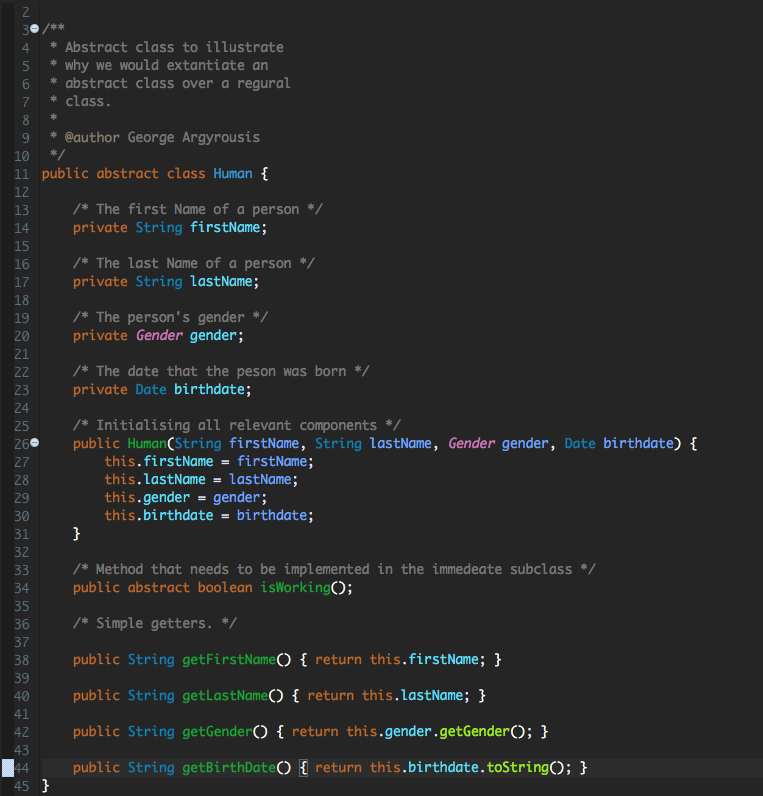
\includegraphics[scale=0.48]{images/Human.png}

            We have defined attributes such as \textit{firstName}, \textit{lastName}, \textit{gender} and \textit{birthdate}. Representing common attributes among all humans. We have also defined one abstract method that will be implemented when the abstract class is extended by another regular class.

            Of course we would not be able to create a \textbf{Human} object.

            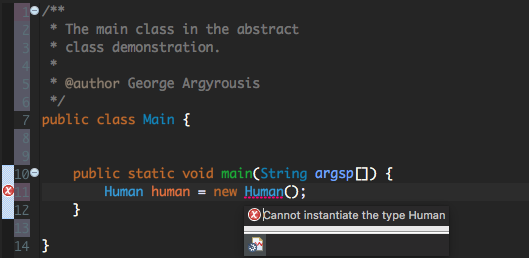
\includegraphics[scale=0.7]{images/Main_error.png}

            Human is an abstract class that has defined general characteristics of the objects we would want in our database. We could possibly have multiple classes such as, \textbf{Professor}, \textbf{Student}, \textbf{Employee} that extend \textbf{Human}.

            Thus inheriting all information provided by the abstract class itself. But we wouldn't want to have Human objects in the database as it is only reflecting the core idea.\\
            We will proceed my making the \textbf{Student} object which extends Human.
            A Student might have multiple other attributes but for this demonstration we will just add two ArrayLists and a StudentID.

            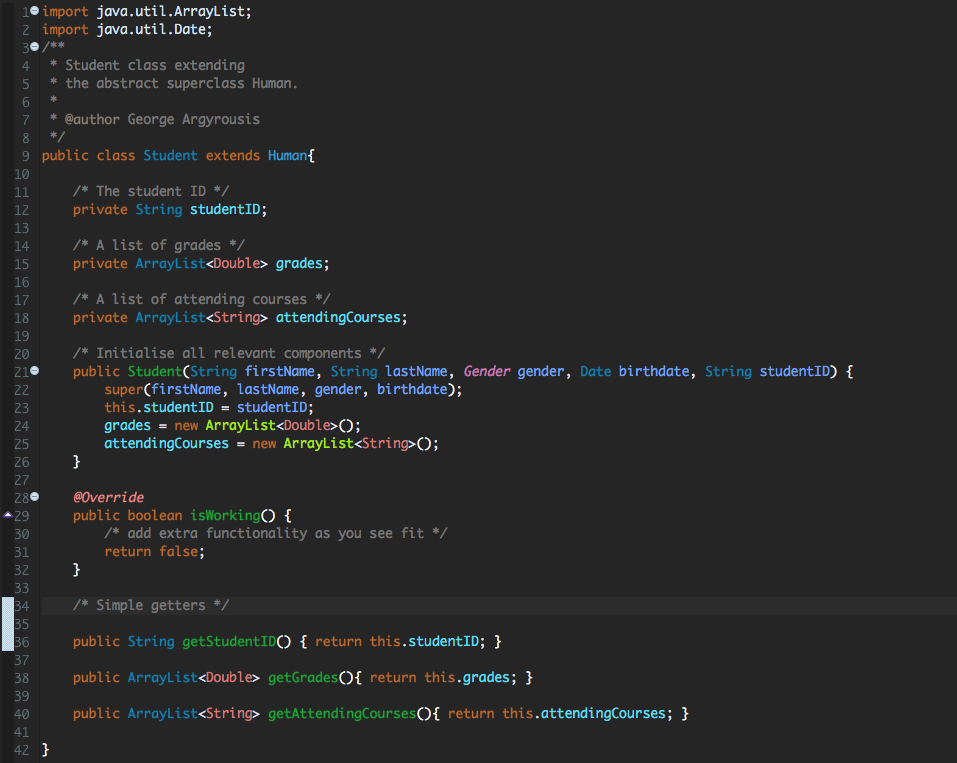
\includegraphics[scale=0.45]{images/Student_Step2.png}

            Last but not least, we initialize the object and print it's attributes in the command line.

            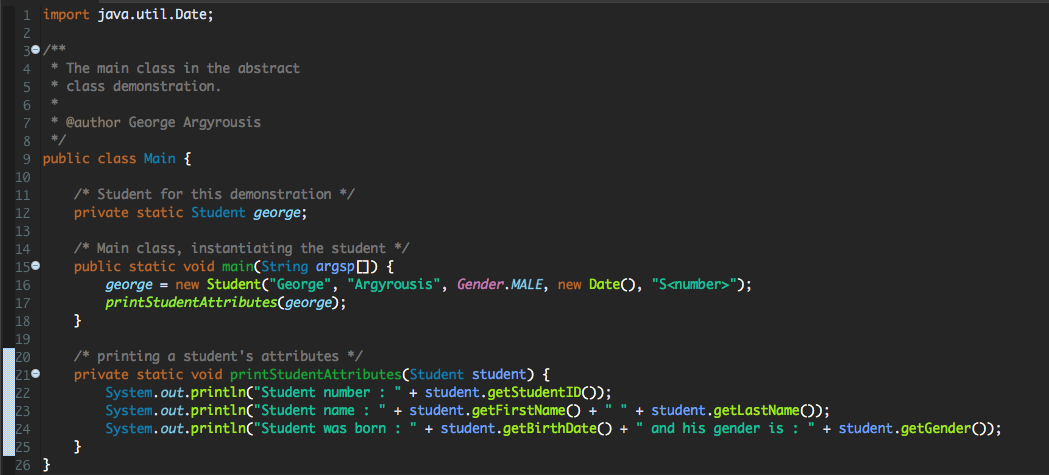
\includegraphics[scale=0.40]{images/Main_without_error.png}

            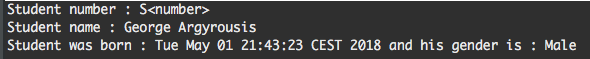
\includegraphics[scale=0.71]{images/output.png}

            To see the source code for this example, and play around with it, check out the \href{https://github.com/andrewlalis/CommandPatternTutorial}{GitHub repository} online!

    \newpage

    \section{Interfaces}
    	\subsection{Definition}
    		\href{https://docs.oracle.com/javase/tutorial/java/concepts/interface.html}{Oracle Java Interface Tutorial}

    		In the most literal sense, an interface is a list of unimplemented methods that should all be related to each other. When an object \textit{implements} an interface, it promises that it will provide behavior for the methods that the interface defines.

    	\subsection{Example}
    		This allows for very useful behavior: Two potentially unrelated classes may implement a common interface, allowing them to be interpreted simply as two arbitrary objects that both have some common methods, thanks to the interface. For example, suppose you are making a video game and need your player to interact with things that have items, like a chest, another player, an NPC, but not with objects such as stones or trees. Without interfaces, we would have have each of these objects inherit from some superclass which defines how to take and give items to these objects. However, conceptually a player is not very related to a tree.

    		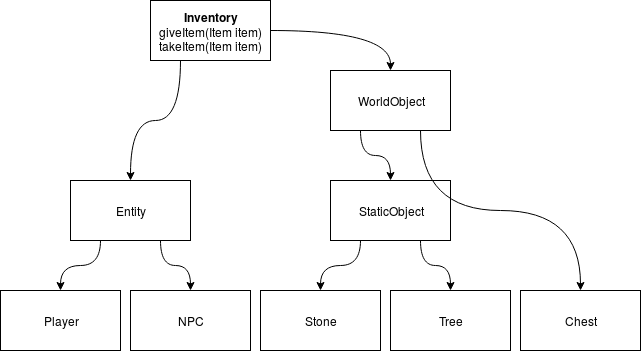
\includegraphics[width=\textwidth]{images/interfaces/classesWithSuperclass.png}

    		To avoid some unintuitive inheritance structure, we can instead introduce an interface which defines methods such as \verb|takeItem(Item item)| and \verb|giveItem(Item item)|. With our new \verb|Tradeable| interface, \textit{or whatever you want to name it, just something descriptive}, each of these objects can now promise that it will implement these methods so that they can be called on a player, a chest, or an NPC.

    		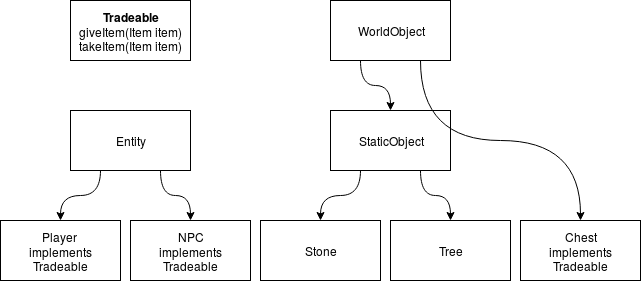
\includegraphics[width=\textwidth]{images/interfaces/classesWithInterface.png}

    	\subsection{Command Pattern}
    		This is only one of many cases where interfaces are the best design choice to make clean, understandable code with a logical type hierarchy. One other application of interfaces is explored in the \href{https://github.com/andrewlalis/CommandPatternTutorial}{command pattern example}. Here, you'll find an example where many \textit{commands} implement the \verb|Command| interface, allowing them to be put in a list and executed arbitrarily. This is useful in many applications and perhaps even the text-based RPG game. Feel free to clone the repository and play around with the code!

    		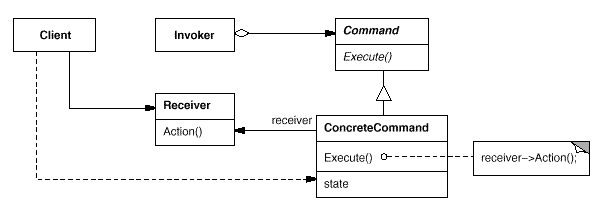
\includegraphics[width=\textwidth]{images/interfaces/commandPattern.png}

	    	\subsubsection{Structure}
	    		In the Command Pattern example, our \verb|Command| interface represents any command that can be applied to a \verb|User| object.

	    		\begin{lstlisting}[language=java]
/**
 * The User class represents some generic object with some instance variables.
 * It acts as the 'receiver' in the command pattern, because the purpose of
 * commands is to modify the receiver.
 */
public class User {

    private String name;
    private int age;
    private boolean online;
	    		\end{lstlisting}

	    		Commands which act on this \verb|User| implement the \verb|Command| interface, shown below.

	    		\begin{lstlisting}[language=java]
public interface Command {

    //Execute some action, with a user object that acts as the receiver.
    void execute(User user);

}
	    		\end{lstlisting}

	    		For simplicity's sake, only one of the \textit{concrete} commands will be shown here. The others are available via the \href{https://github.com/andrewlalis/CommandPatternTutorial}{GitHub repository}.

	    		\begin{lstlisting}[language=java]
public class AgeCommand implements Command {

    @Override
    public void execute(User user) {
        user.setAge(user.getAge()+1);
        System.out.println("User's age has increased to " + user.getAge());
    }
}
	    		\end{lstlisting}

	    		This command, when executed, will increment a given user's age, and print some information about that.

		    \subsubsection{Test it!}
	    		To test these commands, the following code will create a list of all possible commands, then create a user. 10 random commands will be executed on the user, and the output will be printed to the console.

	    		\begin{lstlisting}[language=java]
//Create a list of many commands to execute.
List<Command> commands = new ArrayList<>();

//Add an instance of each type of command.
commands.add(new AgeCommand());
commands.add(new RenameCommand());
commands.add(new ToggleOnlineCommand());

//Random object to select commands.
Random rand = new Random();

//Create a user to act as the receiver. Commands will execute and perform an action on the receiver.
User user = new User("A", 25, false);

//Perform 10 random commands on the user.
for (int i = 0; i < 10; i++){
    Command commandToExecute = commands.get(rand.nextInt(commands.size()));
    commandToExecute.execute(user);
}
	    		\end{lstlisting}

	    		The output of running this is:

	    		\begin{lstlisting}
User's age has increased to 26
User's age has increased to 27
Changed name to: AA
Changed name to: AAAA
User is now online.
User is now offline.
Changed name to: AAAAAAAA
Changed name to: AAAAAAAAAAAAAAAA
Changed name to: AAAAAAAAAAAAAAAAAAAAAAAAAAAAAAAA
User's age has increased to 28
	    		\end{lstlisting}

\end{document}
